\documentclass[conference]{IEEEtran}
\IEEEoverridecommandlockouts
% The preceding line is only needed to identify funding in the first footnote. If that is unneeded, please comment it out.
\usepackage{cite}
\usepackage{amsmath,amssymb,amsfonts}
\usepackage{algorithmic}
\usepackage{graphicx}
\usepackage{url}
\usepackage{caption}
\usepackage{float}
\usepackage{hyperref}\usepackage{adjustbox}
\usepackage{array}

\newcolumntype{R}[2]{%
    >{\adjustbox{angle=#1,lap=\width-(#2)}\bgroup}%
    l%
    <{\egroup}%
}
\newcommand*\rot{\multicolumn{1}{R{90}{-1em}}}% no optional argument here, please!

\def\BibTeX{{\rm B\kern-.05em{\sc i\kern-.025em b}\kern-.08em
    T\kern-.1667em\lower.7ex\hbox{E}\kern-.125emX}}
\begin{document}

\title{Predicting Bitcoin Price using LSTM and Twitter Sentiment Analysis\\
%{\footnotesize \textsuperscript{*}Note: Sub-titles are not captured in Xplore and
%should not be used}
%\thanks{Identify applicable funding agency here. If none, delete this.}
}

\author{\IEEEauthorblockN{}
\IEEEauthorblockA{\textit{Haruki Moriguchi} \\
\textit{haruki.moriguchi@mail.mcgill.ca} \\
ID: 260665818}
\and
\IEEEauthorblockN{}
\IEEEauthorblockA{\textit{Edwin H.Ng} \\
\textit{edwin.ng@mail.mcgill.ca} \\
ID: 260732345}
}

\twocolumn[
  \begin{@twocolumnfalse}
    \maketitle
    \begin{center}
    \begin{minipage}{0.5\linewidth}
    \begin{abstract}
	\textbf{The prediction of stock markets have posed serious challenges to researchers since many factors such as political events, the public opinion and the market trend influence the stock prices. The objective of this paper is to consider the Long Short-Term Memory (LSTM) neural network as a time series model in order to predict the future prices of Bitcoin. LSTM has the advantage of creating dependencies between data that are arbitrarily far apart. The past historical prices of Bitcoin, the volume of tweets related to Bitcoin as well as the sentiment analysis of these tweets will be considered as the inputs of the model. These represents respectively the trend of the Bitcoin price, its popularity, and the public opinion about it.}
\end{abstract}
\begin{IEEEkeywords}
\begin{center}
\textbf{Bitcoin, LSTM, Sentiment Analysis, word2vec}
\end{center}
\end{IEEEkeywords}
    \end{minipage}
    \end{center}
  \end{@twocolumnfalse}
]

\section{Introduction}
\par In recent years, Bitcoin has gained enormous popularity. After receiving many media coverages in 2017, the price went up drastically from 1,000 to 20,000 USD, from which it has since gone down. In fact, this sudden increase in price is not surprising, since behavioral economics states that there are correlations between the public sentiment and the financial market. Fortunately, with the advent of social media, the information about public feelings has become abundant, where Twitter has received a lot of attention from researchers. \\
	The primary contributions of this paper is to test the hypothesis that, in addition to past historical prices, the public sentiment also influences the market. The idea is that although the future movement of a stock price should be a reflection of its past tendencies, the public opinion should also be of important influence to its trajectory. In fact, high pessimism toward a stock should be followed by a downward movement and high optimism should be followed by an upward movement. 
\par The proposed approach is structured as follows. First, a sentimental analysis is  performed on Bitcoin tweets where they are labelled as "negative" or "positive". These results are then fed to a long short-term memory (LSTM) neural network that also learns from the Bitcoin past historical prices in order to predict its future prices. Also fed into the LSTM is the volume of Bitcoin tweets. This is to reflect the growing trend and interest on Bitcoin and of its correlation to the price.
\par	 The data consists of 2,564,353 tweets related to Bitcoin ranging from October 31, 2017 till November 27, 2017.    The Bitcoin price data consists of the hourly prices matching with the corresponding time frame.
	 
 % ------------------------
\section{Related Work}
\par Prediction of stock markets have been proven to be complex and challenging since they are by nature very stochastics. On the one hand, the Efficient-Market hypothesis states that the current price of an asset should be a reflection of all its previous information. On the other hand, the Random-Walk hypothesis claims that the price is independent of its history. Nonetheless, many researchers agree that the prediction of stock markets can be achieved to some degree.  
\par Recently, the LSTM neural networks has gained popularity where it has been used by Nelson et al. \cite{LSTM Stock} to predict the future movement of stock prices. Moreover, LSTM has also gained notoriety as a time series model since it can maintain contextual information as well as temporal behaviours of events. In particular, Zhuge et al. \cite{LSTM Emotional} use the LSTM as a time series model to predict the Shanghai Composite Index based on its historical prices. Furthermore, they have also incorporated an emotional market data into their model in order to reflect the influence of the public opinion on the stock market. The emotional data was obtained throught a sentiment analysis based on a Naive Bayes Classifier that was fed with posts text from Eastmoney with regard to the stocks. Similarly, Khedr et al. \cite{Behavior} have also considered predicting the stock movement through a KNN algorithm that takes into account both its historical prices, and the output of a sentiment analysis based on a Naive Baye Classifier applied to Reuter news. 
\par Another popular source of public opinion is Twitter. In the context of predicting the stock movement through public sentiment, Pagola et al. \cite{word2vec Twitter} introduced the use of Word2Vec in order to textually represent the tweets, whereas the classical approach would be to use the N-gram representation. The former allows for sustainability in word meaning across different contexts.
\par This paper follows the step of \cite{LSTM Emotional} in considering the LSTM as a time series model to predict the future stock prices, based on both historical data and public sentiment. The asset under study in this paper is Bitcoin. The public sentiment will be assessed through another LSTM model that feeds on tweets related to Bitcoin, where they are textually represented through the use of Word2Vec. The volume of tweets is also introduced as another factor impacting the prediction of Bitcoin prices. 


 % ------------------------
\section{Method}

\subsection{Data Collection}
\par The closing prices of Bitcoin have been extracted hourly from October 31, 2017 till November 27, 2017 \footnote{\url{https://bitcoincharts.com}}. Figure \ref{Bitcoin Price} shows the price going in an upward trend from 6,123.21\$ to 9,328.25\$. It is interesting to note that the trend of the volume of tweets, shown in figure \ref{Bitcoin Volume Tweets}, is increasing over that same period as well, suggesting a correlation between the price and the volume of tweets. A total of 2,424,480 tweets related to Bitcoin over the period  of October 31, 2017 till November 27, 2017 are extracted from Twitter API \cite{Twitter API}, using keywords like \# Bitcoin, \# BTC, \# Cryptocurrency, \# Cryptos, etc. 

\begin{minipage}{\linewidth}
\begin{figure}[H]
\centering
\caption{Bitcoin Price from October 31, 2017 till November 27, 2017} 
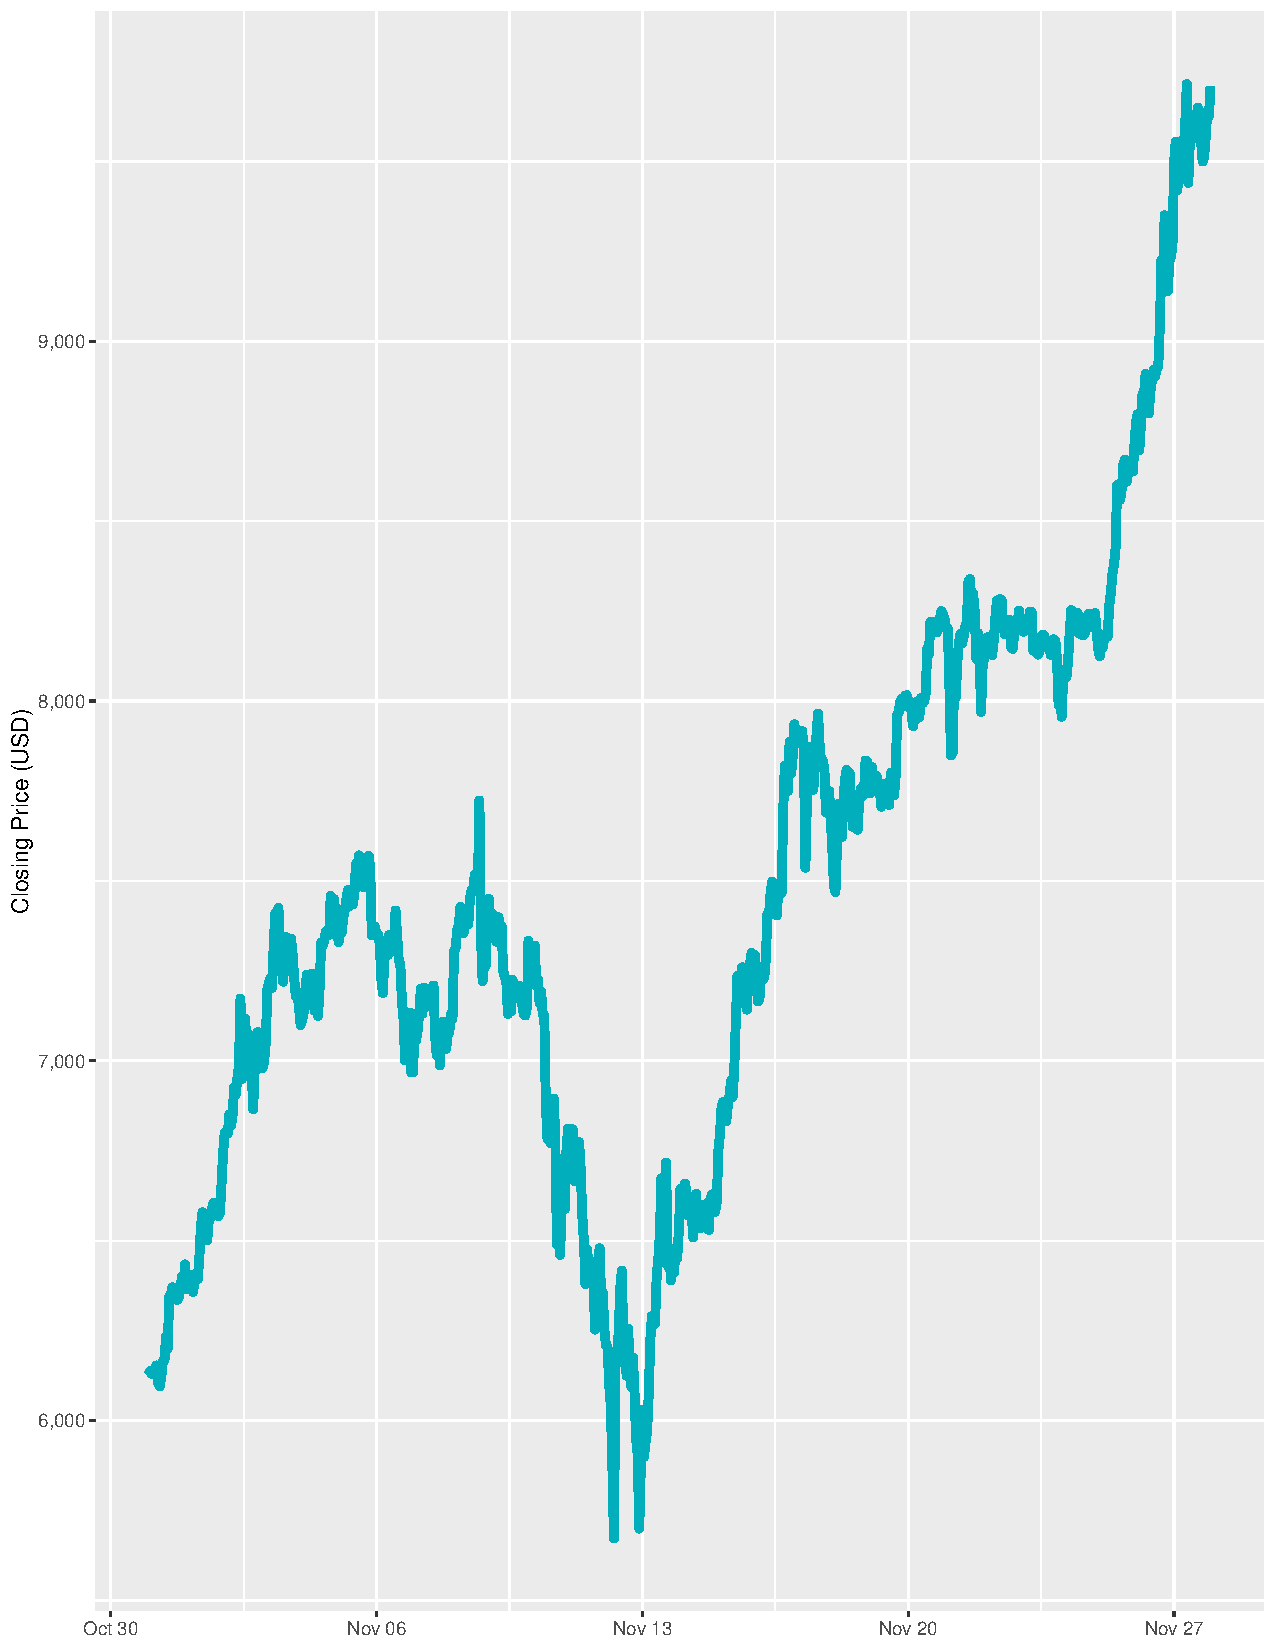
\includegraphics[scale=0.3]{Graphs/BitcoinPriceChart.pdf}
\label{Bitcoin Price} 
\end{figure}
\end{minipage}

\begin{minipage}{\linewidth}
\begin{figure}[H]
\centering
\caption{Bitcoin Volume Tweets from October 31, 2017 till November 27, 2017} 
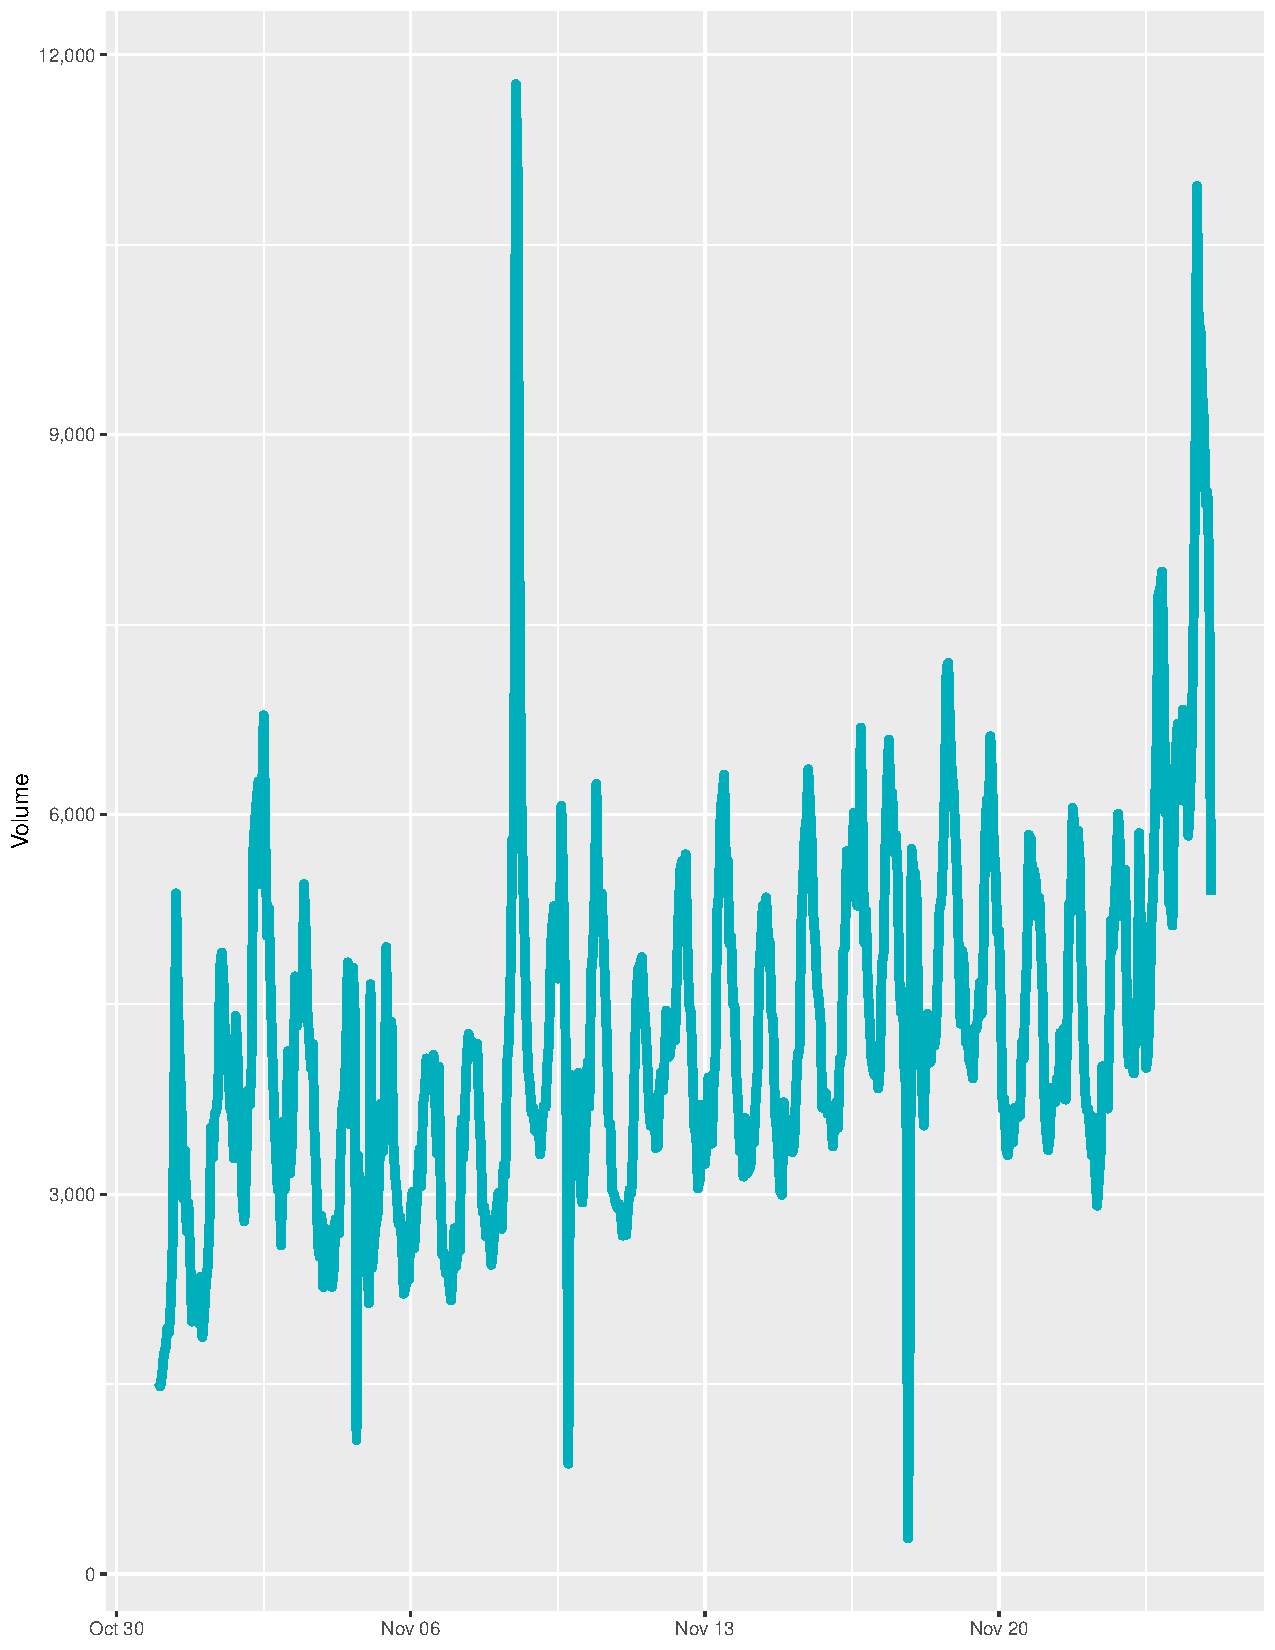
\includegraphics[scale=0.3]{Graphs/BitcoinVolumeChart.pdf}
\label{Bitcoin Volume Tweets} 
\end{figure}
\end{minipage}

\subsection{Pre-processing of the Tweets Data}
\par Tweets are pre-processed in order to filter out the emoticons, and other unnecessary data like URL's. Moreover, they need to be converted into a feacture vector representation. A number of preprocessing steps are taken.
\begin{enumerate}
\item \textit{Tokenization:} Tweets are split into individual words where only alphabetical characters are retained. Using regular expressions, URL's are removed as well. Therefore, each tweet is then a list of the remaining words. Moreover, since LSTM will be used as a sentiment classifier and a uniformed input is needed for the model, tweets are then trimmed down to a maximum of 15 words.

\item \textit{Feature vector representation:} Word2vec is used in order to textually represent each tweet from their list of words. It allows for word embeddings where the meaning of the words are then sustained across different contexts, making the feature vector representation robust. The pre-trained word2vec embeddings from Google\footnote{https://code.google.com/archive/p/word2vec/} is used, which contains 300-dimensional vectors for 3 million words and phrases.
\end{enumerate}

\begin{thebibliography}{2}
\bibitem{Behavior} Khedr, A.E.; Salama, S.E.; Yaseen, N. Predicting Stock Market Behavior using Data Mining Technique and News Sentiment Analysis. \textit{Int. J. Intell. Syst. Appl.} \textbf{2017}, 7, 22-30.
\bibitem{LSTM Stock} Nelson, D. M. Q.; Pereira, A. C. M.; de Oliveira, R. A.. Stock market’s price movement
prediction with LSTM neural networks. \textit{International Joint Conference on Neural Networks (IJCNN)}, \textbf{2017}, 1419-1426.

\bibitem{word2vec Twitter} Pagolu, V. S.; Reddy, K. N.; Ganapati Panda; Majhi, B.. Sentiment
analysis of twitter data for predicting stock market
movements. \textit{International
Conference on Signal Processing, Communication,
Power and Embedded System}, \textbf{2016}, 1345-1350.

\bibitem{LSTM Emotional} Zhuge, Q.; Xu, L.Y.; Zhang, G.W..  LSTM Neural Network with Emotional
Analysis for Prediction of Stock Price. \textit{Engineering Letters}, \textbf{2017}, 25, 167-175.

\bibitem{Twitter API} https://dev.twitter.com/overview/api
\end{thebibliography}




\end{document}
